\documentclass[nojss]{jss}

\title{FFD: Package to substantiate freedom from disease in 
\proglang{R} using two-stage sampling} 

\Plaintitle{FFD: Package to substantiate freedom from disease in R 
using two-stage sampling} 

\Shorttitle{FFD: Freedom From Disease in \proglang{R}} 

\author{Ian Kopacka\\Austrian Agency for Health and Food Safety (AGES)} 
\Plainauthor{Ian Kopacka}

\Address{
  Ian Kopacka\\
  Austrian Agency for Health and Food Safety (AGES)\\
  Division for Data, Statistics and Risk Assessment\\
  Department for EPI-VET\\
  Beethovenstra\ss e 8\\
  A-8010 Graz, Austria\\
  E-mail: \email{ian.kopacka@ages.at}\\
  URL: \url{http://www.ages.at/}
}

\usepackage[utf8]{inputenc}
\usepackage{listings}
\usepackage{tabularx}
\usepackage{makeidx}
\makeindex
\newcolumntype{C}[1]{>{\centering\arraybackslash}p{#1}}   

\newtheorem{example}{Example}[section]
 
\newcommand{\R}{\proglang{R}} \newcommand{\Se}{\mbox{Se}} 
\newcommand{\Sp}{\mbox{Sp}} 


\Abstract{In practise, when conducting surveys to substantiate 
freedom from disease in large populations two-stage sampling 
strategies are often used in order to account for herd-level 
clustering of diseases. Using a modified hypergeometric formula the 
optimal sample size can elegantly be computed, while incorporating 
imperfect diagnostic tests and finite populations; see 
\cite{CaBa98A,CaBa98B}. 

In the package \texttt{FFD}, tools for calculating optimal sample 
sizes (on animal and herd level) using sampling strategies 
``individual sampling'' or ``limited sampling'' (see 
\cite{Ziller02}) are implemented. Further, cost optimal sampling 
strategies, while maintaining constant $\alpha$-levels can be 
computed using \texttt{FFD}. The package furthermore includes tools 
for evaluating the a-posteriori significance ($=1-\alpha$) 
corresponding to a specific sample of herds.} 

\Keywords{\proglang{R}, freedom from disease, sample size 
calculation, individual sampling, limited sampling, a-posteriori 
alpha-error} 
\Plainkeywords{R, freedom from disease, sample size 
calculation, individual sampling, limited sampling, a-posteriori 
alpha-error} 

%%\usepackage{Sweave} %% already provided by jss.cls
%%\VignetteIndexEntry{FFD: Package to substantiate freedom from disease in R}
%%\VignetteDepends{FFD}
%%\VignetteKeywords{R}
%%\VignettePackage{FFD}

\begin{document}

%
%%%%%%%%%%%%%%%%%%%%%%%%%%%%%%%%%%%%%%%%%%%%%%%%%%%%%%%%%%%%%%%%%%%
%%%%%%%%%%%%%%%%%%%%%%%%%%%%%%%%%%%%%%%%%%%%%%%%%%%%%%%%%%%%%%%%%%%
%

%\section*{Note}
%
%The package is still in the pre-alpha phase of development. Not all 
%functionalities are implemented yet. This especially includes 
%methods for sampling using pre-fixed sample sizes, as well as 
%dynamic sampling based on realtime computation of a-posteriori 
%alpha-errors. These features will be included soon. 


\section{Introduction}
\label{sec:introduction}

To meet with standards of trading partners or international 
organizations, it is often required to prove the absence of certain 
diseases in certain animal populations using surveys to substantiate 
freedom from disease. In many cases these surveys are designed in 
two stages: first the number of herds that needs to be tested is 
determined, secondly the number of animals that needs to be tested 
is fixed for each herd. This two-stage sampling accounts for the 
tendency of most diseases to cluster on a herd-level, i.e., the 
characteristics of the spread of a disease within a herd might 
differ from the ability of a disease to spread from one herd to 
another. E.g., there might be a low percentage of infected herds in 
a population, while a herd that is infected might show a rather high 
prevalence. The use of two-stage sampling, however, also has 
practical advantages. In many cases it is not possible to establish 
sampling plans purely on animal-level, as this would require a 
registry of all the animals in the population. Often, such a 
registry only exists for the herds/holdings in an area containing 
only the number of animals per holding (but not a unique identifier 
for those animals). 

The package \texttt{FFD} provides tools to compute the number of 
herds, as well as the number of animals per herd that need to be 
tested using two different sampling schemes that were established in 
\cite{Ziller02}. These schemes are known as \emph{individual 
sampling} and \emph{limited sampling}. For individual sampling the 
number of animals that needs to be tested per herd depends on the 
herd size, while limited sampling uses a pre-fixed number of 
animals, irrespective of the herd size. The advantages and 
disadvantages of the two sampling schemes will be discussed in the 
sections below.  

%
%%%%%%%%%%%%%%%%%%%%%%%%%%%%%%%%%%%%%%%%%%%%%%%%%%%%%%%%%%%%%%%%%%%
%%%%%%%%%%%%%%%%%%%%%%%%%%%%%%%%%%%%%%%%%%%%%%%%%%%%%%%%%%%%%%%%%%%
%

\section{The basics of two-stage sampling} 
\label{sec:2-stage-sampling} 

A survey to substantiate freedom from disease can be regarded as a 
test that is being applied to an entire population. As for a 
diagnostic test, sensitivity and specificity can be determined for 
the survey. The sensitivity of a test is defined as the probability 
of achieving a positive test result, given that the true disease 
status of the tested individual is positive (individual is sick). 
Analogously the specificity of a test is the probability of 
achieving a negative test result, given that the true disease status 
of the tested individual is negative (individual is healthy). 

A typical requirement of a trading partner might be that one must 
show with a probability exceeding 95~\% that no more than 0.2~\% of 
the population is diseased. The probability of establishing a 
prevalence of 0.2~\% or lower reflects the uncertainty that is 
always present due to sampling of a subpopulation only and imperfect 
tests. This percentage is often referred to as the 
\emph{confidence}, while the compliment (1-confidence) is referred 
to as the \emph{significance} $\alpha$. In our case $\alpha = 0.05$. 
The prevalence limit is often referred to as the \emph{design 
prevalence}. 

Now let's look at the survey in the context of sensitivity and 
specificity. The confidence of our survey is the probability of 
finding the disease in a diseased population, i.e., the confidence 
can be regarded as the overall sensitivity of the (statistical) 
test. The specificity of the test is the probability of classifying 
a population as free from the disease, given the population is truly 
free. This parameter is related to the \emph{power} $(1-\beta)$ of 
the test. In surveys substantiating freedom from disease a common 
assumption is that of perfect specificity, i.e., that there are no 
false positives. This assumption on the one hand simplifies the 
computation but it is also practically founded. A positive result 
can have undesired economical implications. It can therefore be 
assumed that all positive results are thoroughly checked using 
multiple tests in order to rule out false positive results.  

%%%%%%%%%%%%%%%%%%%%%%%%%%%%%%%%%%%%%%%%%%%%%%%%%%%%%%%%%%%%%%%%%%%%%%%%%%%%%%%

\subsection{One-stage sampling} 
\label{subsec:1-stage-sampling} 

Let us begin by considering a one-stage sampling scheme for a finite 
population using an imperfect diagnostic test, e.g., let's say we 
consider a herd of animals, and we pick a certain number of animals 
at random. We then test these animals in order to determine if the 
entire herd is infected with a disease or not. In general terms that 
means that we test $n$ individuals from a population with size $N 
\geq n$. If all tested individuals have a negative test result we 
classify the population as being free from the disease. If we find 
one or more individuals that test positive we classify the 
population as diseased. We have to reach a prescribed significance 
$\alpha$, i.e., the probability of finding no testpositives, given 
the population is diseased must be smaller than (or equal to) our 
significance level $\alpha$. In order to compute this probability we 
need to know 

\begin{itemize} \item the population size $N$, \item the sample size 
$n$, \item the prevalence $\pi$ of the disease in the population (or 
the 
      number of diseased individuals in the population $d = N\cdot\pi$) and
\item the sensitivity $\Se$ and the specificity $\Sp$ of the diagnostic test.
\end{itemize}

The probability of finding no testpositives, given that at least $d$ 
individuals are diseased in the population (denoted by $P(T^+=0|d)$) 
can then be computed using a modified hypergeometric formula due to 
\cite{CaBa98A}:

\begin{equation}
\label{eq:hypergeom_senspec_T0} 
% 
P(T^+=0|d) = \sum_{y = \max(0,n-N+d)}^{\min(d,n)} \frac{{d \choose 
y}{N-d \choose n-y}}{{N \choose n}} (1-\Se)^y \Sp^{n-y}. 
% 
\end{equation} 

In the case of perfect specificity the equation is simplified to 
 
\begin{equation}
\label{eq:hypergeom_senspec_T0_simple} 
% 
P(T^+=0|d) = \sum_{y = \max(0,n-N+d)}^{\min(d,n)} \frac{{d \choose 
y}{N-d \choose n-y}}{{N \choose n}} (1-\Se)^y. 
% 
\end{equation} 

In order to compute the optimal sample size one must therefore find 
the smallest sample size $n$, using equation 
(\ref{eq:hypergeom_senspec_T0_simple}), that still satisfies 
$P(T^+=0|d)\leq \alpha$. 

%%%%%%%%%%%%%%%%%%%%%%%%%%%%%%%%%%%%%%%%%%%%%%%%%%%%%%%%%%%%%%%%%%%%%%%%%%%%%%%

\subsection{Two-stage sampling} 
\label{subsec:2-stage-sampling}

The principles of section~\ref{subsec:1-stage-sampling} can easily 
be extended to two-stage sampling; see \cite{CaBa98B}. Instead of 
testing a few animals out of a herd in order to determine the 
disease status of a herd we, e.g., ``test'' a few herds out of a 
larger population in order to determine whether a region or country 
is diseased or not. The only difference is that we cannot directly 
apply a diagnostic test to an entire herd. The so called \emph{herd 
test} rather consists of again picking a certain number of animals 
out of the herd at random and testing those animals using a 
(possibly imperfect) diagnostic test. The sensitivity of the herd 
test is the probability of finding the disease, given the herd is 
infected. As again a herd is considered as diseased if at least one 
animal tests positive, the sensitivity of the herd test is given by 

$$\Se_{herd} = P(T^+>0|d) = 1 - P(T^+ = 0|d) = 1 - \alpha.$$ 

%%%%%%%%%%%%%%%%%%%%%%%%%%%%%%%%%%%%%%%%%%%%%%%%%%%%%%%%%%%%%%%%%%%%%%%%%%%%%%%

\subsubsection{Individual sampling} \label{subsubsec:ind-sampling} 

One way to determine the number of herds to test is to fix a desired 
herd sensitivity, e.g., $\Se_{herd} = 0.7$. That means that for each 
herd that is being tested we have a 70~\% chance of finding the 
disease. For each herd size we can then apply the principles of 
section \ref{subsec:1-stage-sampling} to determine $n$, the number 
of animals we have to test, where $N$ is the herd size, $\alpha = 1 
- \Se_{herd}$ and $d$ is the number of diseased individuals in the 
herds, assuming the herd is infected. This number is related to the 
\emph{intra herd prevalence} $\pi_{IH}$, via $d = N\cdot \pi_{IH}$. 
The intra herd prevalence is usually higher that the design 
prevalence, due to disease clustering on herd-level, and is mostly 
fixed by expert opinions, or determined by surveys.  

\begin{example} \label{ex:ind_sampling1} 

We consider a population of herds where the biggest herd has no more 
than 300 animals. Using a herd sensitivity of $\Se_{herd} = 0.7$, in 
intra herd prevalence of $\pi_{IH} = 0.2$ and a diagnostic test with 
a sensitivity of $90~\%$ the necessary number of animals to test for 
each herd is given in table~\ref{tab:n_ind_sampling1}.

\begin{table}[ht]
\caption{Sample size corresponding to the herd size} 
\begin{center}
\begin{tabular}{c|C{90pt}}\label{tab:n_ind_sampling1} 
\textbf{Herd size} & \textbf{No. of animals to test}\\
\hline 
1 - 3 & entire herd\\
4 - 5 & 4\\
6 & 5\\
7 - 31 & 6\\
32 - 300 & 7\\
\hline
\end{tabular} 
\end{center}
\end{table} 
\end{example} 

The number of herds to test can then again be computed by applying 
the principles of section \ref{subsec:1-stage-sampling}, where $n$ 
is the number of herds to sample, $N$ is the number of herds in the 
population, $\alpha$ is the significance level of the survey, $d$ is 
the number of diseased herds in the population according to the 
design prevalence and $\Se$ is the herd sensitivity. 

\begin{example} \label{ex:ind_sampling2} 

We consider a population of 15000 herds, the biggest of which having 
no more that 300 animals. We need to prove with a confidence of 
95~\% ($\Rightarrow$ significance level $\alpha = 5~\%$) that no 
more than 0.2~\% of the herds are infected, i.e., the design 
prevalence is $\pi = 0.002$. The diagnostic test we are using has a 
sensitivity of 90~\% and the intra-herd prevalence of the disease is 
$\pi_{IH} = 0.2$. 

The parameters above are all determined by the population, the 
infectivity of the disease and by regulations of the trading 
partner. The herd sensitivity, however, can be chosen (almost) 
freely and determines the number of herds and the number of animals 
per herd that need to be sampled. We fix $\Se_{herd} = 0.7$. 

The number of animals tested per herd is then given in 
table~\ref{tab:n_ind_sampling1}. The number of herds to be tested 
can be determined using (\ref{eq:hypergeom_senspec_T0_simple}) with 
$N = 15000$, $\alpha = 0.05$, $\pi = 0.002$ and $\Se = 0.7$. With 
the survey parameters above one needs to draw a sample of 2036 
herds. 

\end{example}  

Note that in the example above the herd sensitivity was fixed. We 
want to stress that, using the methodology above, every herd 
sensitivity chosen within a reasonable range yields a sampling 
scheme satisfying the prescribed significance level. The herd 
sensitivity merely determines the balance between the number of 
animals to test per herd and the number of herds to test and can, 
e.g., be chosen according to economical aspects. 


%%%%%%%%%%%%%%%%%%%%%%%%%%%%%%%%%%%%%%%%%%%%%%%%%%%%%%%%%%%%%%%%%%%%%%%%%%%%%%%

\subsubsection{Limited sampling} \label{subsubsec:ltd-sampling}

Another strategy used for two-stage sampling is \emph{limited 
sampling}. With limited sampling a pre-fixed number of animals $k$ 
(\emph{sample limit}) is tested in each herd, irrespective of the 
herd size. If the herd has fewer animals then the entire herd is 
tested. With this approach the herd sensitivity, i.e., the ability 
to find a disease in a herd, is no longer constant over the 
population (as it is for individual sampling), but depends on the 
herd size. If, e.g., 7 animals are tested out of a herd of 300 then 
the probability of finding a diseased animal is significantly 
smaller than when 7 animals are tested out of a herd of 10 animals. 
Hence, as opposed to individual sampling where the number of animals 
to test varies over the population, while the herd sensitivity is 
constant, for limited sampling the opposite is true. The number of 
animals to test is the same for every herd, but the herd sensitivity 
varies. 

The herd sensitivity $\Se_{herd} = 1 - P(T^+|d)$ can be computed for 
each herd using (\ref{eq:hypergeom_senspec_T0_simple}), where $N$ is 
the herd size, $d=N\cdot \pi_{IH}$, $\Se$ is the sensitivity of the 
diagnostic test and $n=min(N,k)$. 

In order to compute the number of herds to be tested we, however, 
require one fixed herd sensitivity and not - as it is the case here 
- a herd sensitivity depending on the herd size. What is usually 
done is that one uses the mean herd sensitivity 

\begin{equation}
%
\Se_{mean} = \sum_{j = 1}^{N_{max}} \Se_{herd}(N=j,k)\cdot P(N=j),
%
\end{equation}
  
where $N_{max}$ is the biggest herd size in the population, 
$\Se_{herd}(N=j,k)$ is the herd sensitivity of a herd of size $j$ 
using limited sampling with a sample limit $k$ and $P(N=j)$ is the 
proportion of herds with size $j$ in the population, i.e., the 
``probability'' that a herd is of herd size $j$. Using the mean herd 
sensitivity as herd sensitivity the number of herds to be tested can 
again be determined using (\ref{eq:hypergeom_senspec_T0_simple}). 

Similar to the herd sensitivity in individual sampling the sample 
limit determines the balance between the number of animals to test 
per herd and the number of herds to test, while maintaining a 
constant significance level.  

%
%%%%%%%%%%%%%%%%%%%%%%%%%%%%%%%%%%%%%%%%%%%%%%%%%%%%%%%%%%%%%%%%%%%
%%%%%%%%%%%%%%%%%%%%%%%%%%%%%%%%%%%%%%%%%%%%%%%%%%%%%%%%%%%%%%%%%%%
%

\section{Sample size calculation using S4 classes}
%\section{FFD using the S4 classes and methods}
\label{sec:using-ffd-S4}

The package \texttt{FFD} offers convenient tools to compute the 
sample sizes on herd and on animal level for individual and limited 
sampling using S4-classes. With these classes the survey parameters 
need to be specified once, creating an object of the class 
\texttt{SurveyData}. With this object different sampling strategies 
can conveniently be compared with respect to effectivity and costs 
and appropriate strategies can be evaluated and exported as 
html-files.

Furthermore, functions are available to evaluate 
(\ref{eq:hypergeom_senspec_T0_simple}), find the optimal sample 
sizes on herd and animal level, to evaluate herd sensitivities for 
limited sampling etc. These functions operate with conventional 
R-classes (vectors, data frames) and, while the use is not as 
convenient as with the methods for the S4 classes, they offer a 
greater flexibility. 

%%%%%%%%%%%%%%%%%%%%%%%%%%%%%%%%%%%%%%%%%%%%%%%%%%%%%%%%%%%%%%%%%%%

\subsection{Specifying the survey parameters}
\label{subsec:surveyData} 

The following parameters/data are required in order to fix the 
sample size: 

\begin{itemize} 
% 
\item \texttt{nAnimalVec}: A vector of herd sizes (=number of
animals in a herd). Each component of the vector corresponds to a herd 
in the population,
\item \texttt{designPrevalence}: The prevalence threshold in the population
that the survey must establish,
\item \texttt{alpha}: Significance level of the survey (= 1 - confidence),
\item \texttt{intraHerdPrevalence}: The assumed prevalence of the 
disease within an infected herd,
\item \texttt{diagSensitivity}: The sensitivity of the diagnostic test.
%
\end{itemize} 

If it is desired to optimize the sampling strategy with respect to 
overall costs, parameters \texttt{costHerd}, \texttt{costAnimal}, 
describing the cost of each tested herd (excluding the cost per 
tested animal) and the cost of each tested animal, respectively. The 
overall costs are then computed using the simple model:

$$\mbox{cost = number of tested herds * cost per herd + number of 
tested animals * cost per animal}.$$ 
 
The cost per tested animal, e.g., contain the cost of drawing and 
analyzing the sample. The cost per tested herd could contain the 
travel costs of the vet etc.

All the survey parameters are packed into an S4 object of the class 
\texttt{SurveyData} \index{Class!\texttt{SurveyData}} 
\index{\texttt{SurveyData}}  using the constructor 
\texttt{surveyData()}. \index{\texttt{surveyData()}} Additionally, 
further population data, such as herd identifiers, names and 
addresses of the owners etc. can be passed to the constructor in the 
form of a data frame, where each row of the data frame corresponds 
to a component of the vector \texttt{nAnimalVec}. 

In the following example the data set \texttt{sheepData}, contained 
in the package \texttt{FFD}, is used. The data set contains 
simulated data resembling the sheep holdings in Austria. 

 

\begin{Schunk}
\begin{Sinput}
> data(sheepData) 
> mySurvey <- surveyData(nAnimalVec = sheepData$nSheep, 
       populationData = sheepData, designPrevalence = 0.002, 
       alpha = 0.05, intraHerdPrevalence = 0.2, 
       diagSensitivity = 0.9, costHerd = 30, costAnimal = 7) 
> summary(mySurvey)    
\end{Sinput}
\begin{Soutput}
Survey Parameters:
------------------
Design Prevalence:               0.002 
Significance level:              0.05 
Intra herd prevalence:           0.20 
Sensitivity of diagnostic test:  0.90 
Cost per tested herd:            30.00 
Cost per tested animal:          7.00 

Survey Data:
------------
Number of herds:             15287 
Total number of animals:     224606 
Number of animals per herd: 
   Min. 1st Qu.  Median    Mean 3rd Qu.    Max. 
   1.00    4.00    8.00   14.69   17.00  249.00 
Additional population data: 
'data.frame':	15287 obs. of  3 variables:
 $ herdId: int  1 2 3 4 5 6 7 8 9 10 ...
 $ state : int  7 7 6 3 8 7 3 7 4 3 ...
 $ nSheep: num  22 30 4 11 11 3 94 53 4 24 ...
\end{Soutput}
\end{Schunk}

\index{Method!\texttt{summary-SurveyData}} 
\index{Method!\texttt{show-SurveyData}} Objects of the class 
\texttt{SurveyData} are the basic building blocks used in the 
package \texttt{FFD}, containing all the necessary data for the 
design of an appropriate sampling scheme using individual or limited
sampling. 

%%%%%%%%%%%%%%%%%%%%%%%%%%%%%%%%%%%%%%%%%%%%%%%%%%%%%%%%%%%%%%%%%%%

\subsection{Individual sampling} 
\label{subsec:ind-sampling}

With individual sampling the number of animals to test per herd in
order to achieve a specified herd sensitivity depends on the herd
size. The herd sensitivity, hence, determines the number of animals
to test per herd, as well as the number of herd to test, while
maintaining a constant overall significance level $\alpha$. If a low
herd sensitivity is chosen the number of animals to test per herd is
low, while the number of herds to test might be rather high. If,
however a high herd sensitivity is specified the number of animals
tested per herd increases, while the number of herds to test
decreases. If the cost per tested herd and the cost per tested
animal is known a herd sensitivity might be chosen in order to
minimize the overall costs of the survey.

\subsubsection{Cost optimization}

The package \texttt{FFD} provides the S4-class
\texttt{IndSamplingSummary}
\index{Class!\texttt{IndSamplingSummary}}
\index{\texttt{IndSamplingSummary}} and the function
\texttt{indSamplingSummary()}, \index{\texttt{indSamplingSummary()}}
as a convenient tool to minimize the survey costs for individual
sampling. The class constructor \texttt{indSamplingSummary()} takes
an object of the class \texttt{SurveyData} and a step size for the
herd sensitivities as an argument and computes the number of herds
to test, the expected total number of animals tested based on the
herd size distribution in the population, as well as the expected
overall costs of the survey for a sequence of herd sensitivities. The
herd sensitivities range from 0.1 to the sensitivity of the
diagnostic test, the step size for the discretization is either
specified by the user or a default value of 0.02 is used.

\begin{Schunk}
\begin{Sinput}
> myIndSamplingSummary <- indSamplingSummary(survey.Data = mySurvey, 
       stepSize = 0.05)
> summary(myIndSamplingSummary)
\end{Sinput}
\begin{Soutput}
INDIVIDUAL SAMPLING:

Survey Parameters:
------------------
Design Prevalence:               0.002 
Significance level:              0.05 
Intra herd prevalence:           0.20 
Sensitivity of diagnostic test:  0.90 
Cost per tested herd:            30.00 
Cost per tested animal:          7.00 

Survey Data:
------------
Number of herds:             15287 
Total number of animals:     224606 
Number of animals per herd: 
   Min. 1st Qu.  Median    Mean 3rd Qu.    Max. 
   1.00    4.00    8.00   14.69   17.00  249.00 
Additional population data: 
'data.frame':	15287 obs. of  3 variables:
 $ herdId: int  1 2 3 4 5 6 7 8 9 10 ...
 $ state : int  7 7 6 3 8 7 3 7 4 3 ...
 $ nSheep: num  22 30 4 11 11 3 94 53 4 24 ...

Cost optimal sampling strategy:
-------------------------------
Herd sensitivity:                          0.90 
Number of herds to test:                   1564 
Expected total number of animals to test:  10743.38 
Expected total costs of the survey:        122123.67 
\end{Soutput}
\end{Schunk}

\index{Method!\texttt{summary-IndSamplingSummary}}
\index{Method!\texttt{show-IndSamplingSummary}} A plot of the object
of class \texttt{IndSamplingSummary} can be created using
\texttt{plot()}. \index{Method!\texttt{plot-IndSamplingSummary}} The
plot consists of (row-wise from top left to bottom right)

\begin{itemize}
\item the mean number of animals to test per herd plotted against the herd sensitivity,
\item the number of herds to test plotted against the herd sensitivity,
\item the expected total number of animals to test plotted against the herd sensitivity,
\item the expected overall costs plotted against the herd sensitivity.
\end{itemize}

\setkeys{Gin}{width=15cm}
\begin{Schunk}
\begin{Sinput}
> plot(myIndSamplingSummary)
\end{Sinput}
\end{Schunk}
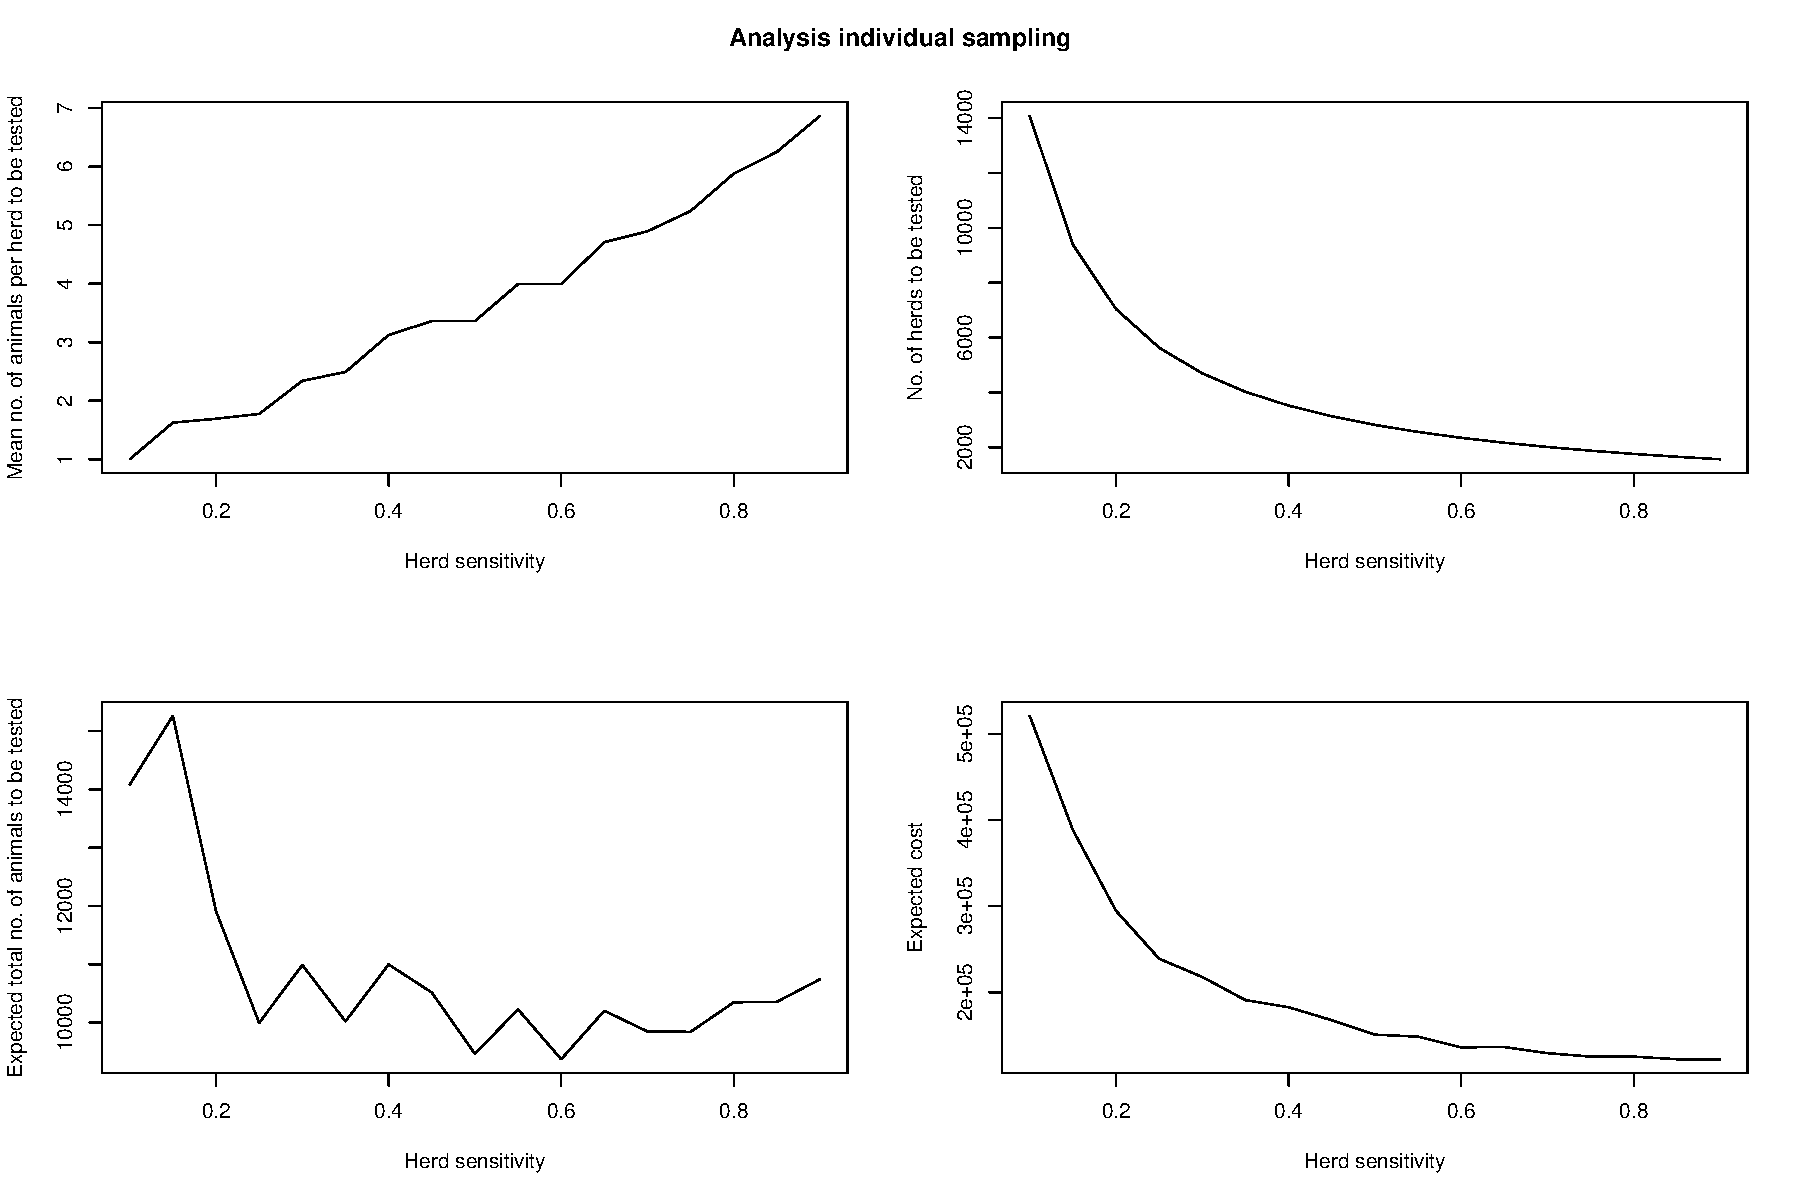
\includegraphics{FFD-intro-004}

The summary of the object of class \texttt{IndSamplingSummary} can
further be exported to an html-file using the method \texttt{HTML}.
\index{Method!\texttt{HTML-IndSamplingSummary}} This requires the
specification of a file to write to, which can be done using the
function \texttt{HTMLInitFile()} from the package \texttt{R2HTML}.

\begin{Schunk}
\begin{Sinput}
> target <- HTMLInitFile(getwd(), filename = "IndSampling")
> HTML(myIndSamplingSummary)
> HTMLEndFile()
\end{Sinput}
\end{Schunk} 


\subsubsection{Parameters for a fixed herd sensitivity}

If one has decided on an appropriate herd sensitivity, number of 
herds to test, the expected total number of animals to test, the 
expected costs and a lookup table containing the number of animals 
to test per herd depending on the herd size can be computed using 
the function \texttt{indSampling()} \index{\texttt{indSampling()}} 
to create an object of the class \texttt{IndSampling}. 
\index{Class!\texttt{IndSampling}} \index{\texttt{IndSampling}} The 
function takes two arguments, \texttt{survey.Data}, an object of the 
class \texttt{SurveyData}, and the herd sensitivity 
\texttt{herdSensitivity}. The computed parameters can again be 
displayed using the methods \texttt{show()}, \texttt{summary()} and 
\texttt{HTML()}. \index{Method!\texttt{show-IndSampling}} 
\index{Method!\texttt{summary-IndSampling}} 
\index{Method!\texttt{HTML-IndSampling}} 

For a herd sensitivity of 0.7 the parameters are:
  
\begin{Schunk}
\begin{Sinput}
> myIndSampling <- indSampling(survey.Data = mySurvey, 
       herdSensitivity = 0.7)
> summary(myIndSampling) 
\end{Sinput}
\begin{Soutput}
INDIVIDUAL SAMPLING:

Survey Parameters:
------------------
Design Prevalence:               0.002 
Significance level:              0.05 
Intra herd prevalence:           0.20 
Sensitivity of diagnostic test:  0.90 
Cost per tested herd:            30.00 
Cost per tested animal:          7.00 

Survey Data:
------------
Number of herds:             15287 
Total number of animals:     224606 
Number of animals per herd: 
   Min. 1st Qu.  Median    Mean 3rd Qu.    Max. 
   1.00    4.00    8.00   14.69   17.00  249.00 
Additional population data: 
'data.frame':	15287 obs. of  3 variables:
 $ herdId: int  1 2 3 4 5 6 7 8 9 10 ...
 $ state : int  7 7 6 3 8 7 3 7 4 3 ...
 $ nSheep: num  22 30 4 11 11 3 94 53 4 24 ...

Sampling strategy:
------------------
Herd sensitivity:                          0.70 
Number of herds to test:                   2011 
Expected total number of animals to test:  9845.44 
Expected total costs of the survey:        129248.09 
Lookup table for the number of animals to test per herd:

   Herd size  |  No. of animals to test 
   ------------------------------------ 
     1 - 3    |       entire herd       
     4 - 5    |            4            
       6      |            5            
    7 - 31    |            6            
   32 - 249   |            7            
\end{Soutput}
\end{Schunk}

%%%%%%%%%%%%%%%%%%%%%%%%%%%%%%%%%%%%%%%%%%%%%%%%%%%%%%%%%%%%%%%%%%%

\subsection{Limited sampling} 
\label{subsec:ltd-sampling} 

For limited sampling a pre-fixed number of animals per selected herd 
(=the sample limit) is tested, irrespective of the actual herd size. 
The chosen sample limit determines the (mean) herd sensitivity and 
thus the sample size on a herd level. The sample limit and the 
number of herds act in a complementary fashion in the sense that low 
sampling limits result in a large number of herds to be tested and 
vice versa. If the cost per tested herd and the cost per tested 
animal is known the package can be used to find the cost optimal 
sample limit. 

\subsubsection{Cost optimization}

The package \texttt{FFD} provides the S4-class 
\texttt{LtdSamplingSummary} 
\index{Class!\texttt{LtdSamplingSummary}} 
\index{\texttt{LtdSamplingSummary}} and the function 
\texttt{ltdSamplingSummary()}, \index{\texttt{ltdSamplingSummary()}} 
where the mean herd sensitivity, the number of herds to test, the 
expected total number of animals tested based on the herd size 
distribution in the population, as well as the expected overall 
costs of the survey is computed for a sequence of sample limits. The 
smallest considered sample limit is 1 animal per herd, the largest 
sample limit can be specified by the user via the argument 
\texttt{sampleSizeLtdMax}, or if no upper bound is specified, the 
largest herd size is used. 

\begin{Schunk}
\begin{Sinput}
> myLtdSampleSummary = ltdSamplingSummary(survey.Data = mySurvey,
       sampleSizeLtdMax = 30)
> summary(myLtdSampleSummary)
\end{Sinput}
\begin{Soutput}
LIMITED SAMPLING:

Survey Parameters:
------------------
Design Prevalence:               0.002 
Significance level:              0.05 
Intra herd prevalence:           0.20 
Sensitivity of diagnostic test:  0.90 
Cost per tested herd:            30.00 
Cost per tested animal:          7.00 

Survey Data:
------------
Number of herds:             15287 
Total number of animals:     224606 
Number of animals per herd: 
   Min. 1st Qu.  Median    Mean 3rd Qu.    Max. 
   1.00    4.00    8.00   14.69   17.00  249.00 
Additional population data: 
'data.frame':	15287 obs. of  3 variables:
 $ herdId: int  1 2 3 4 5 6 7 8 9 10 ...
 $ state : int  7 7 6 3 8 7 3 7 4 3 ...
 $ nSheep: num  22 30 4 11 11 3 94 53 4 24 ...

Cost optimal sampling strategy:
-------------------------------
Fixed number of animals to test per herd:  5 
Mean herd sensitivity:                     0.77 
Number of herds to test:                   1830 
Expected total number of animals to test:  7854.38 
Expected total costs of the survey:        109880.68 
\end{Soutput}
\end{Schunk}
 
\index{Method!\texttt{summary-LtdSamplingSummary}} 
\index{Method!\texttt{show-LtdSamplingSummary}} A plot of the object 
of class \texttt{LtdSamplingSummary} can be created using 
\texttt{plot()}. \index{Method!\texttt{plot-LtdSamplingSummary}} The 
plot consists of (row-wise from top left to bottom right) 

\begin{itemize}
\item the mean herd sensitivity plotted against the sample limit,
\item the number of herds to test plotted against the sample limit,
\item the expected total number of animals to test plotted against the sample limit,
\item the expected overall costs plotted against the sample limit.
\end{itemize}

\setkeys{Gin}{width=15cm}
\begin{Schunk}
\begin{Sinput}
> plot(myLtdSampleSummary)  
\end{Sinput}
\end{Schunk}
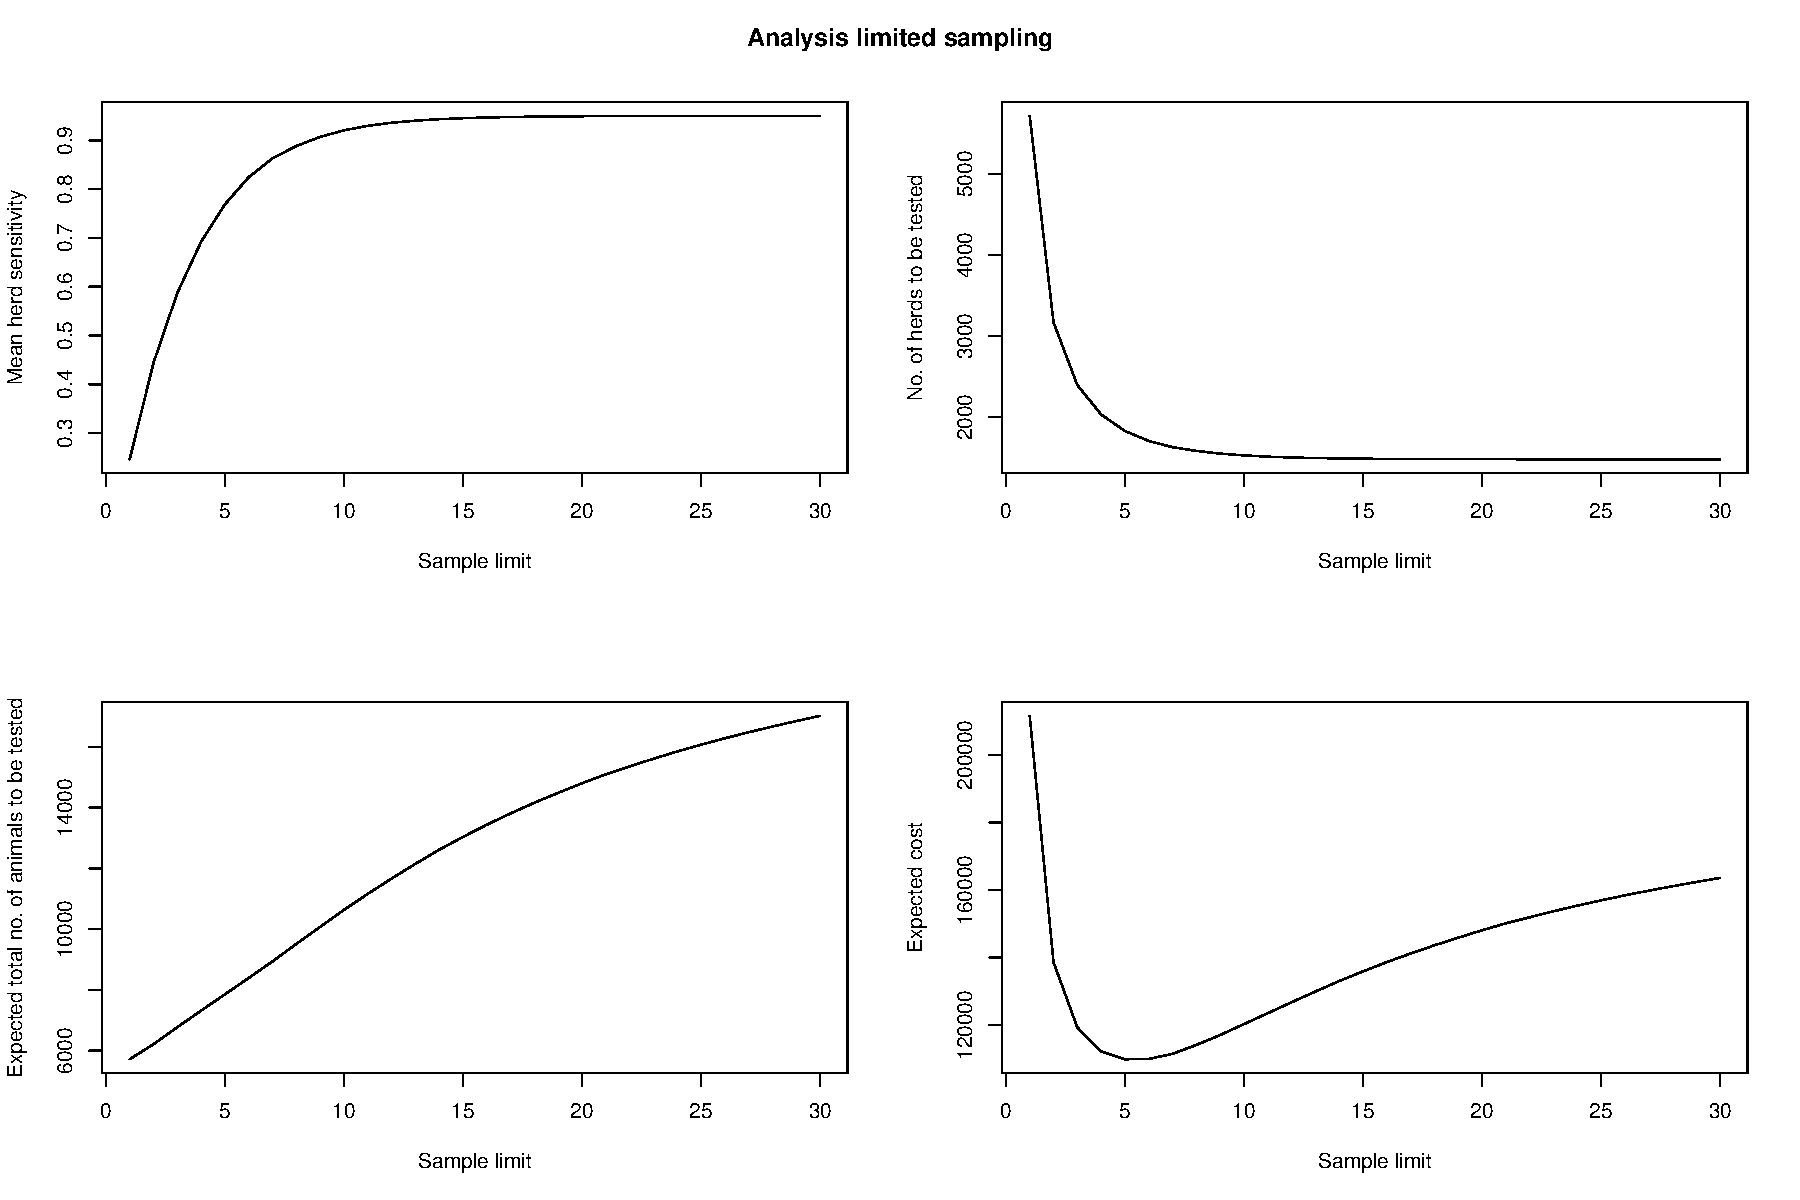
\includegraphics{FFD-intro-007}

The summary of the object of class \texttt{LtdSamplingSummary} can 
further be exported to an html-file using the method \texttt{HTML}. 
\index{Method!\texttt{HTML-LtdSamplingSummary}} This requires the 
specification of a file to write to, which can be done using the 
function \texttt{HTMLInitFile()} from the package \texttt{R2HTML}. 

\begin{Schunk}
\begin{Sinput}
> target <- HTMLInitFile(getwd(), filename = "LtdSampling")
> HTML(myLtdSamplingSummary)
> HTMLEndFile()
\end{Sinput}
\end{Schunk} 

\subsubsection{Parameters for a fixed sample limit}

If one has decided on an appropriate sample size the herd 
sensitivity, number of herds to test, expected total number of 
animals to test and expected costs can be determined using the 
function \texttt{ltdSampling()} \index{\texttt{ltdSampling()}} to 
create an object of the class \texttt{LtdSampling}. 
\index{Class!\texttt{LtdSampling}} \index{\texttt{LtdSampling}} The 
function takes two arguments, \texttt{survey.Data}, an object of the 
class \texttt{SurveyData}, and the sample limit 
\texttt{sampleSizeLtd}. The computed parameters can again be 
displayed using the methods \texttt{show()}, \texttt{summary()} and 
\texttt{HTML()}. \index{Method!\texttt{show-LtdSampling}} 
\index{Method!\texttt{summary-LtdSampling}} 
\index{Method!\texttt{HTML-LtdSampling}} 

Let's say we have chosen the appropriate sample limit to be 7 
animals per herd: 
  
\begin{Schunk}
\begin{Sinput}
> myLtdSampling <- ltdSampling(survey.Data = mySurvey, 
       sampleSizeLtd = 7)
> summary(myLtdSampling) 
\end{Sinput}
\begin{Soutput}
LIMITED SAMPLING:

Survey Parameters:
------------------
Design Prevalence:               0.002 
Significance level:              0.05 
Intra herd prevalence:           0.20 
Sensitivity of diagnostic test:  0.90 
Cost per tested herd:            30.00 
Cost per tested animal:          7.00 

Survey Data:
------------
Number of herds:             15287 
Total number of animals:     224606 
Number of animals per herd: 
   Min. 1st Qu.  Median    Mean 3rd Qu.    Max. 
   1.00    4.00    8.00   14.69   17.00  249.00 
Additional population data: 
'data.frame':	15287 obs. of  3 variables:
 $ herdId: int  1 2 3 4 5 6 7 8 9 10 ...
 $ state : int  7 7 6 3 8 7 3 7 4 3 ...
 $ nSheep: num  22 30 4 11 11 3 94 53 4 24 ...

Sampling strategy:
------------------
Fixed number of animals to test per herd:  7 
Mean herd sensitivity:                     0.86 
Number of herds to test:                   1630 
Expected total number of animals to test:  8939.78 
Expected total costs of the survey:        111478.48 
\end{Soutput}
\end{Schunk}


%
%%%%%%%%%%%%%%%%%%%%%%%%%%%%%%%%%%%%%%%%%%%%%%%%%%%%%%%%%%%%%%%%%%%
%%%%%%%%%%%%%%%%%%%%%%%%%%%%%%%%%%%%%%%%%%%%%%%%%%%%%%%%%%%%%%%%%%%
%

\section{Sample size calculation without classes}
\label{sec:using-ffd-noclass}

In order to provide sufficient flexibility \texttt{FFD} offers a set 
of tools that operate with traditional data types (mostly vectors 
and data frames). The basis of these tools is equation 
(\ref{eq:hypergeom_senspec_T0}), the evaluation of which is 
implemented in the function \texttt{computePValue}. 
\index{\texttt{computePValue()}} The function takes the population 
size, the sample size, the number of diseased individuals in the 
population, the sensitivity and the specificity of the test as 
arguments and returns the probability of finding no testpositive 
individuals, given that the disease is present in the population 
with the design prevalence: 

\begin{Schunk}
\begin{Sinput}
> p.value <- computePValue(nPopulation = 15287, nSample = 1630, 
       nDiseased = round(15287*0.002), sensitivity = 0.8633, specificity = 1)
> p.value
\end{Sinput}
\begin{Soutput}
[1] 0.04997705
\end{Soutput}
\end{Schunk}

The optimal sample size is defined as the smallest sample size that 
still produces a probability smaller than a given significance 
level. This sample size can be evaluated using the function 
\texttt{computeOptimalSampleSize}. 
\index{\texttt{computeOptimalSampleSize()}}The function takes the 
population size, the design prevalence, the significance level, the 
sensitivity and the specificity of the test as arguments (the 
argument \texttt{lookupTable} will be discussed in section 
\ref{subsec:ind-sampling-noclass} on individual sampling) and 
returns the optimal sample size: 

\begin{Schunk}
\begin{Sinput}
> nSample <- computeOptimalSampleSize(nPopulation = 15287, 
       prevalence = 0.002, alpha = 0.05, sensitivity = 0.8633, 
       specificity = 1, lookupTable = FALSE)
> nSample 
\end{Sinput}
\begin{Soutput}
[1] 1630
\end{Soutput}
\end{Schunk}


%%%%%%%%%%%%%%%%%%%%%%%%%%%%%%%%%%%%%%%%%%%%%%%%%%%%%%%%%%%%%%%%%%%
\subsection{Individual sampling} \label{subsec:ind-sampling-noclass}

For individual sampling the herd sensitivity is fixed and constant 
for every sampled herd. Hence the number of herds to test can be 
computed using \texttt{computeOptimalSampleSize}. The arguments are 
the number of herds in the population (\texttt{nPopulation}), the 
design prevalence of the survey (\texttt{prevalence}), the desired 
overall significance level (\texttt{alpha}) and the herd sensitivity 
(\texttt{sensitivity}). The specificity should be 1 and 
\texttt{lookupTable} is set to \texttt{FALSE}. 

The number of animals to test for each herd using individual 
sampling can be computed using the function 
\texttt{computeOptimalSampleSize} by setting the switch 
\texttt{lookupTable} to \texttt{TRUE}. The function then produces a 
lookup table in the form of a matrix. The input arguments are the 
maximal herd size that should be included in the  lookup table 
(\texttt{nPopulation}), the intra herd prevalence 
(\texttt{prevalence}), 1 - the desired herd sensitivity 
(\texttt{alpha}), the sensitivity of the diagnostic test 
(\texttt{sensitivity}) and the specificity of the diagnostic test 
(\texttt{specificity}), which should be kept at 1. 

\begin{Schunk}
\begin{Sinput}
> lookupTable <- computeOptimalSampleSize(nPopulation = max(sheepData$nSheep), 
       prevalence = 0.2, alpha = 0.3, sensitivity = 0.9, 
       specificity = 1, lookupTable = TRUE)
> lookupTable 
\end{Sinput}
\begin{Soutput}
     N_lower N_upper sampleSize
[1,]       1       1          1
[2,]       2       2          2
[3,]       3       3          3
[4,]       4       5          4
[5,]       6       6          5
[6,]       7      31          6
[7,]      32     249          7
\end{Soutput}
\end{Schunk}


%%%%%%%%%%%%%%%%%%%%%%%%%%%%%%%%%%%%%%%%%%%%%%%%%%%%%%%%%%%%%%%%%%%

\subsection{Limited sampling} \label{subsec:ltd-sampling-noclass}  

For limited sampling the herd sensitivity depends on the herd size. 
The herd size is complementary to the significance level $\alpha$ of 
the herd test, i.e., herd sensitivity = 1 - $\alpha$. The 
$\alpha$-values of the herd test, as well as the mean $\alpha$ (= 1 
- mean herd sensitivity) is computed via the function 
\texttt{computeAlphaLimitedSampling()}. 
\index{\texttt{computeAlphaLimitedSampling()}} The function takes a 
vector containing the herd sizes for each holding, the sample limit, 
the intra herd prevalence and sensitivity and specificity of the 
diagnostic test and returns a list with two elements. The first 
element \texttt{alphaDataFrame} is a data frame with columns 
\texttt{size} and \texttt{alpha} containing the alpha-errors 
(=1-herd sensitivity) for each herd size. The second element 
\texttt{meanAlpha} is the mean of the alpha values corresponding to 
the herd size distribution in the population: 

\begin{Schunk}
\begin{Sinput}
> alphaList <- computeAlphaLimitedSampling(stockSizeVector = sheepData$nSheep, 
       sampleSizeLtd = 7, intraHerdPrevalence = 0.2, diagSensitivity = 0.9, 
       diagSpecificity = 1)
> str(alphaList$alphaDataFrame) 
\end{Sinput}
\begin{Soutput}
'data.frame':	173 obs. of  2 variables:
 $ size : num  1 2 3 4 5 6 7 8 9 10 ...
 $ alpha: num  0.1 0.1 0.1 0.1 0.1 0.1 0.1 0.0325 0.0725 0.118 ...
\end{Soutput}
\begin{Sinput}
> alphaList$meanAlpha 
\end{Sinput}
\begin{Soutput}
[1] 0.1367245
\end{Soutput}
\end{Schunk}

The number of herds to be tested can then be computed using 
\texttt{computeOptimalSampleSize}. The arguments are the number of 
herds in the population (\texttt{nPopulation}), the design 
prevalence of the survey (\texttt{prevalence}), the desired overall 
significance level (\texttt{alpha}), the mean herd sensitivity = 1 - 
\texttt{alphaList\$meanAlpha} (\texttt{sensitivity}). The specificity and 
\texttt{lookupTable} should be kept at their default values.


%
%%%%%%%%%%%%%%%%%%%%%%%%%%%%%%%%%%%%%%%%%%%%%%%%%%%%%%%%%%%%%%%%%%%
%%%%%%%%%%%%%%%%%%%%%%%%%%%%%%%%%%%%%%%%%%%%%%%%%%%%%%%%%%%%%%%%%%%
%

\section{A-posteriori calculation of the alpha-error}
\label{sec:aposteriori}

The calculation of the sample size on herd level, i.e., the number 
of herds to test is based on the herd sensitivity. For limited 
sampling the herd sensitivity depends on the size of each herd, 
hence a mean herd sensitivity is used for the sample size 
calculation. This, on the other hand, means that the overall 
significance level of the scheme depends on the chosen sample, i.e., 
if the sample contains a high proportion of very large herds the 
mean herd sensitivity in the sample is lower than the mean herd 
sensitivity in the population and hence the desired overall 
significance level is not met. If the sample contains a lot of very 
small herds, then the mean herd sensitivity in the sample exceeds 
that of the population and the significance of the sampling scheme 
falls below the desired significance level, i.e., the sampling 
scheme is ``too thorough'', more herds are being tested than 
necessary. 

It is therefore of interest to compute the significance level of the 
sampling scheme after the sample has been drawn, i.e., to compute 
the a-posteriori alpha-error, which is the probability of finding no 
testpositives in the \textbf{given sample}, given that the disease 
is present at the design prevalence. The a-posteriori alpha-error 
can then be used to assess a given sample and to possibly modify it, 
i.e., reduce or extend it in order to meet the prescribed 
significance level. 

The a-posteriori analysis of the alpha-error is also of interest 
when using individual sampling. With individual sampling the number 
of animals to test is computed for every herd size, in order to 
guarantee the ``same'' herd sensitivity for every herd. The herd 
sensitivity as a function of the number of animals tested is however 
a discrete function with jumps. The exact value can in most cases 
not be achieved and the desired herd sensitivity is taken as a lower 
bound, i.e., for each herd the number of animals to test is computed 
as the smallest number that achieves a herd sensitivity greater or 
equal to the desired value. E.g., for a herd of a given size the 
herd sensitivity when testing 4 animals might be 0.68 and for 5 
animals it might be 0.74. If the desired herd sensitivity is 0.7 
then 5 animals would be tested. The mean herd sensitivity for 
individual sampling therefore always exceeds the desired value, 
hence the number of herds to test is generally higher than 
necessary. 

The package \texttt{FFD} offers tools to compute the a-posteriori 
alpha-error for a given sample. Furthermore a sampling scheme is 
implemented that dynamically updates the a-posteriori alpha-error 
during the sampling procedure and updates the sample size 
automatically in order to prevent under- or overestimation of the 
sample size. 

%%%%%%%%%%%%%%%%%%%%%%%%%%%%%%%%%%%%%%%%%%%%%%%%%%%%%%%%%%%%%%%%%%% 
\subsection{Computation of the a-posteriori alpha-error using FFD} 

The a-posteriori error of a given sample can be computed using the 
function \texttt{computeAposterioriError()}. 
\index{\texttt{computeAposterioriError()}} The function requires the 
population size, the number of diseased elements in the population 
according to the design prevalence and a vector of the herd-level 
alpha-errors of the herds in the sample (= 1 - herd sensitivity). 
Furthermore it can be specified if the a-posteriori error should be 
computed exactly or if an approximation should be used. The exact 
calculation is computationally costly due to combinatorial issues 
and is not recommended if there are more than 6 diseased elements in 
the population. The approximation comes very close to the exact 
value and is significantly more efficient. 

The vector of herd-level alpha-errors can be generated using the 
function \texttt{computeAlpha()}. \index{\texttt{computeAlpha()}} It 
takes the vector of herd sizes, the intra herd prevalence, the 
sensitivity of the diagnostic test as arguments, as well as 
parameters concerning the sample strategy: for \texttt{method == 
"limited"} the sample limit \texttt{sampleSizeLtd} must be 
specified, for \texttt{method == "individual"} the herd sensitivity 
\texttt{herdSensitivity} must be specified:

\begin{Schunk}
\begin{Sinput}
> sampleVec <- sample(sheepData$nSheep, 2550, replace = FALSE)
> alphaVec <- computeAlpha(nAnimalVec = sampleVec,
      method = "limited", sampleSizeLtd = 9,
      intraHerdPrevalence = 0.2, diagSensitivity = 0.9)
> system.time({
   errorExact <- computeAposterioriError(alphaErrorVector = alphaVec, 
       nPopulation = 5000, nDiseased = 5, method = "exact")})
\end{Sinput}
\begin{Soutput}
   user  system elapsed 
   0.33    0.00    0.33 
\end{Soutput}
\begin{Sinput}
> errorExact    
\end{Sinput}
\begin{Soutput}
[1] 0.04461766
\end{Soutput}
\begin{Sinput}
> system.time({
   errorApprox <- computeAposterioriError(alphaErrorVector = alphaVec, 
       nPopulation = 5000, nDiseased = 5, method = "approx")})
\end{Sinput}
\begin{Soutput}
   user  system elapsed 
      0       0       0 
\end{Soutput}
\begin{Sinput}
> errorApprox
\end{Sinput}
\begin{Soutput}
[1] 0.04461784
\end{Soutput}
\end{Schunk}


%%%%%%%%%%%%%%%%%%%%%%%%%%%%%%%%%%%%%%%%%%%%%%%%%%%%%%%%%%%%%%%%%%%

\subsection{Sampling using S4 classes} 
\label{subsec:sampling_with_class}

The method \texttt{sample()} 
\index{Method!\texttt{sample-IndSampling}}\index{Method!\texttt{sample-LtdSampling}} 
has been implemented for the classes \texttt{IndSampling} and 
\texttt{IndSampling}. It takes two arguments, the first argument 
\texttt{x} is an object of the class \texttt{IndSampling} or 
\texttt{LtdSampling} and the second argument \texttt{size} is a 
character string specifying the sampling strategy. For \texttt{size 
= "fixed"} the fixed number \texttt{x@nHerds} of herds is sampled 
using simple random sampling. For \texttt{size = "dynamic"} dynamic 
sampling is used. The method returns a list with two items: a vector 
of indices of the sampled herds corresponding to 
\texttt{x@surveyData@nAnimalVec} and the a-posteriori alpha-error of 
the sample:

\begin{Schunk}
\begin{Sinput}
> ## Fixed sampling:
> ##################
> sampleFixed <- sample(x = myIndSampling, size = "fixed")
> ## Sample Size:
> length(sampleFixed$indexSample)
\end{Sinput}
\begin{Soutput}
[1] 2011
\end{Soutput}
\begin{Sinput}
> ## Significance:
> sampleFixed$aPostAlpha
\end{Sinput}
\begin{Soutput}
[1] 0.03027402
\end{Soutput}
\begin{Sinput}
> ## Dynamic sampling:
> ####################
> sampleDynamic <- sample(x = myIndSampling, size = "dynamic")
> ## Sample Size:
> length(sampleDynamic$indexSample)
\end{Sinput}
\begin{Soutput}
[1] 1741
\end{Soutput}
\begin{Sinput}
> ## Significance:
> sampleDynamic$aPostAlpha
\end{Sinput}
\begin{Soutput}
[1] 0.04998022
\end{Soutput}
\end{Schunk}
  

%%%%%%%%%%%%%%%%%%%%%%%%%%%%%%%%%%%%%%%%%%%%%%%%%%%%%%%%%%%%%%%%%%%
%\tableofcontents

\printindex

\bibliography{FFD}

\end{document}


%%% Local Variables: 
%%% mode: latex
%%% TeX-master: t
%%% End: 
